\section{Sở GD\&ĐT Quảng Ninh 25--26, Lần 2}

\caulc
\Opensolutionfile{ans}[ans/ans-04-26-2-QuangNinh-SoGD-LC]

\begin{ex}%[1D2N2-2]
	Trong bốn dãy số sau, có bao nhiêu dãy số lập thành một cấp số cộng?
	\begin{itemize}
		\item[I)] $10, -2, -14, -26, -38$.
		\item[II)] $\dfrac{1}{2}, \dfrac{5}{4}, 2, \dfrac{11}{4}, \dfrac{7}{2}$.
		\item[III)] $\sqrt{1}, \sqrt{2}, \sqrt{3}, \sqrt{4}, \sqrt{5}$.
		\item[IV)] $1, 4, 7, 10, 13$.
	\end{itemize}
	\choice
	{$1$}
	{$2$}
	{\True $3$}
	{$4$}
	\loigiai{
		Ta xét từng dãy số:
		\begin{itemize}
			\item Dãy I: $-2-10 = -14 - \left( -2 \right) = -26 - \left( -14 \right) = -38 - \left( -26 \right) = -12$. Đây là cấp số cộng có công sai $d=-12$.
			\item Dãy II: $\dfrac{5}{4} - \dfrac{1}{2} = 2 - \dfrac{5}{4} = \dfrac{11}{4} - 2 = \dfrac{7}{2} - \dfrac{11}{4} = \dfrac{3}{4}$. Đây là cấp số cộng có công sai $d=\dfrac{3}{4}$.
			\item Dãy III: $\sqrt{2} - \sqrt{1} \neq \sqrt{3} - \sqrt{2}$. Đây không phải là cấp số cộng.
			\item Dãy IV: $4-1 = 7-4 = 10-7 = 13-10 = 3$. Đây là cấp số cộng có công sai $d=3$.
		\end{itemize}
		Vậy có $3$ dãy số lập thành cấp số cộng.
	}
\end{ex}

\begin{ex}%[1D1N5-3] 
	Phương trình $\sin x = 0$ có họ nghiệm là
	\choice
	{$x = \dfrac{\pi}{2} + k2\pi, k \in \mathbb{Z}$}
	{$x = k2\pi, k \in \mathbb{Z}$}
	{$x = \dfrac{\pi}{2} + k\pi, k \in \mathbb{Z}$}
	{\True $x = k\pi, k \in \mathbb{Z}$}
	\loigiai{
		Phương trình cơ bản: $\sin x = 0 \Leftrightarrow x = k\pi, k \in \mathbb{Z}$.
	}
\end{ex}

\begin{ex}%[1D6N2-1]
	Với mọi số thực dương $a$ thì $\log_2 \left( 16a \right) - \log_2 a$ bằng
	\choice
	{$\log_2 \left( 15a \right)$}
	{$8$}
	{\True $4$}
	{$4 - 2\log_2 a$}
	\loigiai{
		Ta có: $\log_2 \left( 16a \right) - \log_2 a = \log_2 \left( \dfrac{16a}{a} \right) = \log_2 16 = 4$.
	}
\end{ex}

\begin{ex}%[1H8H7-2]
	Cho hình chóp $S.ABC$ có đáy $ABC$ là tam giác vuông tại $B$ và cạnh bên $SA$ vuông góc với đáy, biết $AB = a$, $AC = 2a$, $SA = a\sqrt{3}$. Thể tích khối chóp $S.ABC$ bằng
	\choice
	{\True $\dfrac{1}{2}a^3$}
	{$\dfrac{3}{2}a^3$}
	{$\dfrac{\sqrt{3}}{3}a^3$}
	{$\dfrac{\sqrt{3}}{2}a^3$}
	\loigiai{
		Tam giác $ABC$ vuông tại $B$, theo định lý Pytago ta có:
		$BC = \sqrt{AC^2 - AB^2} = \sqrt{\left( 2a \right)^2 - a^2} = a\sqrt{3}$.
		Diện tích tam giác đáy $ABC$ là: $S_{\Delta ABC} = \dfrac{1}{2}AB \cdot BC = \dfrac{1}{2}a \cdot a\sqrt{3} = \dfrac{a^2\sqrt{3}}{2}$.
		Thể tích khối chóp $S.ABC$ là: $V = \dfrac{1}{3}S_{\Delta ABC} \cdot SA = \dfrac{1}{3} \cdot \dfrac{a^2\sqrt{3}}{2} \cdot a\sqrt{3} = \dfrac{1}{2}a^3$.
	}
\end{ex}

\begin{ex}%[2H2H1-2]
	Cho hình chóp $S.ABCD$ có đáy là hình bình hành tâm $O$. Đẳng thức nào sau đây sai?
	\choice
	{$\overrightarrow{AB} + \overrightarrow{AD} = \overrightarrow{AC}$}
	{\True $\overrightarrow{SA} + \overrightarrow{SB} = \overrightarrow{SC} + \overrightarrow{SD}$}
	{$\overrightarrow{SA} + \overrightarrow{SC} = 2\overrightarrow{SO}$}
	{$\overrightarrow{SB} + \overrightarrow{SD} = 2\overrightarrow{SO}$}
	\loigiai{
		Do $ABCD$ là hình bình hành tâm $O$ nên $O$ là trung điểm của $AC$ và $BD$.
		Theo tính chất trung điểm, ta có:
		$\overrightarrow{SA} + \overrightarrow{SC} = 2\overrightarrow{SO}$ và $\overrightarrow{SB} + \overrightarrow{SD} = 2\overrightarrow{SO}$.
		Do đó $\overrightarrow{SA} + \overrightarrow{SC} = \overrightarrow{SB} + \overrightarrow{SD}$.
		Đẳng thức $\overrightarrow{SA} + \overrightarrow{SB} = \overrightarrow{SC} + \overrightarrow{SD}$ là sai.
	}
\end{ex}

\begin{ex}%[2D1N4-1]
	Cho hàm số $y=f(x)$ xác định và liên tục trên $\mathbb{R} \setminus \left\{ -1 \right\}$, có bảng biến thiên như sau.
	\begin{center}
		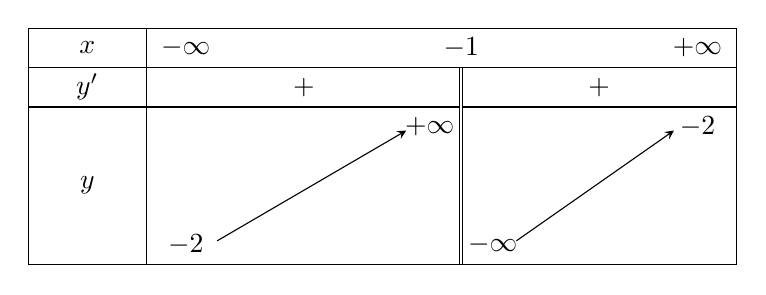
\begin{tikzpicture}[>=stealth, scale=1]
			\draw (0,0) rectangle (9,3);
			\draw (0,2) -- (9,2);
			\draw (0,2.5) -- (9,2.5);
			\draw (1.5,0) -- (1.5,3);
			\node at (0.75, 2.75) {$x$};
			\node at (0.75, 2.25) {$y'$};
			\node at (0.75, 1) {$y$};
			\node at (2, 2.75) {$-\infty$};
			\node at (5.5, 2.75) {$-1$};
			\node at (8.5, 2.75) {$+\infty$};
			\draw[double, distance=2pt] (5.5,0) -- (5.5,2.5);
			\node at (3.5, 2.25) {$+$};
			\node at (7.25, 2.25) {$+$};
			\node at (2, 0.25) {$-2$};
			\node at (5.1, 1.75) {$+\infty$};
			\draw[->] (2.4, 0.3) -- (4.8, 1.7);
			\node at (5.9, 0.25) {$-\infty$};
			\node at (8.5, 1.75) {$-2$};
			\draw[->] (6.2, 0.3) -- (8.2, 1.7);
		\end{tikzpicture}
	\end{center}
	Khẳng định nào sau đây là đúng?
	\choice
	{Đồ thị hàm số có tiệm cận đứng $y = -1$ và tiệm cận ngang $x = -2$}
	{Đồ thị hàm số có duy nhất một tiệm cận}
	{Đồ thị hàm số có ba tiệm cận}
	{\True Đồ thị hàm số có tiệm cận đứng $x = -1$ và tiệm cận ngang $y = -2$}
	\loigiai{
		Dựa vào bảng biến thiên, ta có:
		$\lim\limits_{x \to -1^-} f(x) = +\infty$ và $\lim\limits_{x \to -1^+} f(x) = -\infty$ suy ra đường thẳng $x = -1$ là tiệm cận đứng của đồ thị hàm số.
		$\lim\limits_{x \to -\infty} f(x) = -2$ và $\lim\limits_{x \to +\infty} f(x) = -2$ suy ra đường thẳng $y = -2$ là tiệm cận ngang của đồ thị hàm số.
		Vậy đồ thị hàm số có tiệm cận đứng $x = -1$ và tiệm cận ngang $y = -2$.
	}
\end{ex}

\begin{ex}%[2D1H2-1]
	Hàm số $y = f(x) = x^3 - 3x^2 - 9x + 7$ có cực đại là
	\choice
	{$-1$}
	{\True $12$}
	{$3$}
	{$-20$}
	\loigiai{
		Tập xác định: $D = \mathbb{R}$.
		Ta có $y' = 3x^2 - 6x - 9$.
		Cho $y' = 0 \Leftrightarrow 3x^2 - 6x - 9 = 0 \Leftrightarrow x = -1$ hoặc $x = 3$.
		Bảng biến thiên:
		\begin{center}
			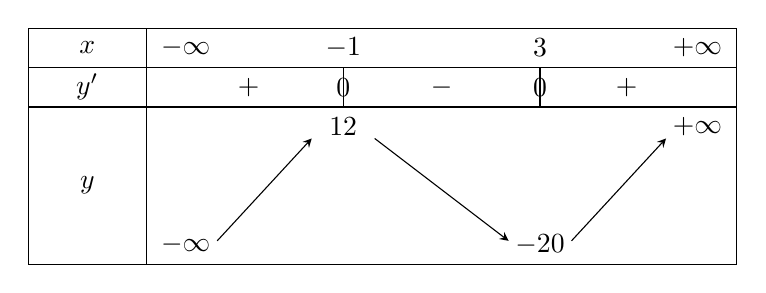
\begin{tikzpicture}[>=stealth, scale=1]
				\draw (0,0) rectangle (9,3);
				\draw (0,2) -- (9,2);
				\draw (0,2.5) -- (9,2.5);
				\draw (1.5,0) -- (1.5,3);
				\node at (0.75, 2.75) {$x$};
				\node at (0.75, 2.25) {$y'$};
				\node at (0.75, 1) {$y$};
				\node at (2, 2.75) {$-\infty$};
				\node at (4, 2.75) {$-1$};
				\node at (6.5, 2.75) {$3$};
				\node at (8.5, 2.75) {$+\infty$};
				\draw (4,2) -- (4,2.5);
				\draw (6.5,2) -- (6.5,2.5);
				\node at (4, 2.25) {$0$};
				\node at (6.5, 2.25) {$0$};
				\node at (2.8, 2.25) {$+$};
				\node at (5.25, 2.25) {$-$};
				\node at (7.6, 2.25) {$+$};
				\node at (2, 0.25) {$-\infty$};
				\node at (4, 1.75) {$12$};
				\node at (6.5, 0.25) {$-20$};
				\node at (8.5, 1.75) {$+\infty$};
				\draw[->] (2.4, 0.3) -- (3.6, 1.6);
				\draw[->] (4.4, 1.6) -- (6.1, 0.3);
				\draw[->] (6.9, 0.3) -- (8.1, 1.6);
			\end{tikzpicture}
		\end{center}
		Dựa vào bảng biến thiên, hàm số đạt cực đại tại điểm $x = -1$ và giá trị cực đại của hàm số là $12$.
	}
\end{ex}

\begin{ex}%[2D4N1-4]
	Họ nguyên hàm của hàm số $f(x)=2025^x$ là
	\choice
	{$F(x)=2025^x+C$}
	{\True $F(x)=\dfrac{2025^x}{\ln\left( 2025 \right)}+C$}
	{$F(x)=2025.2024^x+C$}
	{$F(x)=2025x+C$}
	\loigiai{
		Ta có họ nguyên hàm của hàm số đã cho là $\int 2025^x \mathrm{d}x = \dfrac{2025^x}{\ln\left( 2025 \right)} + C$.
	}
\end{ex}

\begin{ex}%[1D5N2-2]
	Kết quả kiểm tra điểm môn Toán của học sinh lớp 12A1 được cho bởi mẫu số liệu ghép nhóm như sau:
	\begin{center}
		\begin{tabular}{|l|c|c|c|c|c|}
			\hline
			Nhóm điểm & $\left[ 0;2 \right)$ & $\left[ 2;4 \right)$ & $\left[ 4;6 \right)$ & $\left[ 6;8 \right)$ & $\left[ 8;10 \right)$ \\
			\hline
			Tần số & $4$ & $5$ & $6$ & $25$ & $10$ \\
			\hline
		\end{tabular}
	\end{center}
	Trung vị của mẫu số liệu ghép nhóm trên thuộc vào nhóm nào dưới đây?
	\choice
	{\True $\left[ 6;8 \right)$}
	{$\left[ 2;4 \right)$}
	{$\left[ 4;6 \right)$}
	{$\left[ 8;10 \right)$}
	\loigiai{
		Cỡ mẫu $n = 4 + 5 + 6 + 25 + 10 = 50$.
		Gọi $x_1, x_2, \dots, x_{50}$ là điểm số của $50$ học sinh được xếp theo thứ tự không giảm.
		Trung vị của mẫu số liệu là trung bình cộng của giá trị thứ $25$ và $26$: $\dfrac{x_{25}+x_{26}}{2}$.
		Ta có:
		\begin{itemize}
			\item $4$ giá trị đầu tiên thuộc nhóm $\left[ 0;2 \right)$.
			\item $5$ giá trị tiếp theo thuộc nhóm $\left[ 2;4 \right)$.
			\item $6$ giá trị tiếp theo thuộc nhóm $\left[ 4;6 \right)$.
			\item $25$ giá trị tiếp theo thuộc nhóm $\left[ 6;8 \right)$.
		\end{itemize}
		Do $4+5+6 = 15$ và $15+25=40$ nên $x_{25}$ và $x_{26}$ đều thuộc nhóm $\left[ 6;8 \right)$.
		Vậy trung vị thuộc nhóm $\left[ 6;8 \right)$.
	}
\end{ex}

\begin{ex}%[2H5N1-1]
	Trong không gian $Oxyz$, mặt phẳng $\left( Oxz \right)$ có phương trình là
	\choice
	{\True $y=0$}
	{$z=0$}
	{$x=0$}
	{$x+y+z=0$}
	\loigiai{
		Trong không gian $Oxyz$, mặt phẳng $\left( Oxz \right)$ vuông góc với trục $Oy$ tại gốc tọa độ nên có phương trình là $y=0$.
	}
\end{ex}

\begin{ex}%[2H5N2-1] 
	Trong không gian $Oxyz$, cho đường thẳng $d \colon \dfrac{x-2}{1} = \dfrac{y-1}{-2} = \dfrac{z+1}{3}$. Điểm nào dưới đây thuộc đường thẳng $d$?
	\choice
	{$Q\left( 2;1;1 \right)$}
	{$M\left( 1;2;3 \right)$}
	{\True $P\left( 2;1;-1 \right)$}
	{$N\left( 1;-2;3 \right)$}
	\loigiai{
		Thay tọa độ điểm $P\left( 2;1;-1 \right)$ vào phương trình đường thẳng $d$ ta được:
		$\dfrac{2-2}{1} = \dfrac{1-1}{-2} = \dfrac{-1+1}{3} = 0$ (luôn đúng).
		Vậy $P\left( 2;1;-1 \right) \in d$.
	}
\end{ex}

\begin{ex}%[2H5N3-3] 
	Trong không gian $Oxyz$, phương trình mặt cầu $\left( S \right)$ tâm $I\left( -2;1;0 \right)$ và có đường kính bằng $8$ là
	\choice
	{$\left( S \right) \colon \left( x+2 \right)^2+\left( y-1 \right)^2+z^2=8$}
	{\True $\left( S \right) \colon \left( x+2 \right)^2+\left( y-1 \right)^2+z^2=16$}
	{$\left( S \right) \colon \left( x-2 \right)^2+\left( y+1 \right)^2+z^2=64$}
	{$\left( S \right) \colon \left( x+2 \right)^2+\left( y-1 \right)^2+z^2=64$}
	\loigiai{
		Mặt cầu $\left( S \right)$ có đường kính bằng $8 \Rightarrow$ bán kính mặt cầu là $R = \dfrac{8}{2} = 4$.
		Phương trình mặt cầu $\left( S \right)$ có tâm $I\left( -2;1;0 \right)$ và bán kính $R=4$ là:
		$\left( x+2 \right)^2+\left( y-1 \right)^2+z^2 = 4^2 \Leftrightarrow \left( x+2 \right)^2+\left( y-1 \right)^2+z^2=16$.
	}
\end{ex}

\Closesolutionfile{ans}

\cauds
\Opensolutionfile{ans}[ans/ans-04-26-2-QuangNinh-SoGD-DS]


\begin{ex}%[2D1H5-7]
	Cho hàm số $y=f\left( x \right)=\dfrac{x^2-x-12}{x-2}$.
	\choiceTF
	{\True Đồ thị hàm số $f\left( x \right)$ đi qua điểm $\left( 4;0 \right)$}
	{Đồ thị hàm số $f\left( x \right)$ có đường tiệm cận xiên là đường thẳng $y=x-1$}
	{\True Đồ thị hàm số $f\left( x \right)$ có tâm đối xứng là điểm $I\left( 2;3 \right)$}
	{\True Phương trình đường tiếp tuyến của đồ thị hàm số $f\left( x \right)$ tại điểm $x=3$ có dạng $y=mx+n$, giá trị $m-n$ bằng $50$}
	\loigiai{
		\begin{itemchoice}
			\itemch Thay $x=4$ vào hàm số, ta có $f\left( 4 \right)=\dfrac{4^2-4-12}{4-2}=0$. Vậy đồ thị hàm số $f\left( x \right)$ đi qua điểm $\left( 4;0 \right)$.
			\itemch Ta có $y=\dfrac{x^2-x-12}{x-2}=x+1-\dfrac{10}{x-2}$. Vì $\lim\limits_{x \to +\infty} \left[ y-\left( x+1 \right) \right]=\lim\limits_{x \to +\infty} \left( -\dfrac{10}{x-2} \right)=0$ nên đồ thị hàm số có đường tiệm cận xiên là đường thẳng $y=x+1$.
			\itemch Đồ thị hàm số có đường tiệm cận đứng là $x=2$ và đường tiệm cận xiên là $y=x+1$. Giao điểm của hai đường tiệm cận là tâm đối xứng của đồ thị. Tọa độ tâm đối xứng $I$ là nghiệm của hệ $\begin{cases} x=2 \\ y=x+1 \end{cases} \Rightarrow I\left( 2;3 \right)$.
			\itemch Tập xác định: $D=\mathbb{R} \setminus \left\{ 2 \right\}$. Ta có $f'\left( x \right)=1+\dfrac{10}{\left( x-2 \right)^2}$. Tại $x_0=3$, tung độ tiếp điểm là $y_0=f\left( 3 \right)=3+1-\dfrac{10}{3-2}=-6$ và hệ số góc của tiếp tuyến là $k=f'\left( 3 \right)=1+\dfrac{10}{\left( 3-2 \right)^2}=11$. Phương trình tiếp tuyến tại $x=3$ là $y=11\left( x-3 \right)-6 \Leftrightarrow y=11x-39$. Suy ra $m=11$ và $n=-39$. Vậy $m-n=11-\left( -39 \right)=50$.
		\end{itemchoice}
	}
\end{ex}

\begin{ex}%[2D4H1-6]
	Trong một nhà máy, tốc độ tiêu thụ điện năng của một dây chuyền sản xuất sau khi khởi động có xu hướng giảm dần theo thời gian và tiến về mức ổn định. Giả sử sau khi bắt đầu vận hành được $t$ giờ, tốc độ tiêu thụ điện năng của dây chuyền sản xuất này được mô hình bởi hàm số $E'(t) = A + \mathrm{e}^{-0{,}4t}$ (đơn vị: kWh/giờ) $\left( 0 \le t \le 8 \right)$, trong đó $E(t)$ (kWh) là lượng điện năng tiêu thụ tính từ lúc bắt đầu vận hành. Biết rằng trong $8$ giờ đầu tiên, dây chuyền đã tiêu thụ tổng cộng $120$ kWh.
	\choiceTF
	{\True $E(t) = At - \dfrac{5}{2}\mathrm{e}^{-0{,}4t} + C$, với $C$ là hằng số}
	{$A = 14$ (kết quả làm tròn đến hàng đơn vị)}
	{Lượng điện năng tiêu thụ của dây chuyền trong $4$ giờ đầu lớn hơn $65$ kWh}
	{Tốc độ tiêu thụ điện năng trung bình của dây chuyền sản xuất trong khoảng thời gian từ $a$ giờ đến $b$ giờ được xác định bởi công thức $\overline{v} = \dfrac{E(b) - E(a)}{b - a}$ (kWh/giờ). Tốc độ tiêu thụ điện năng trung bình của dây chuyền sản xuất này trong $4$ giờ cuối bằng $14{,}6$ kWh/giờ (kết quả làm tròn đến hàng phần mười)}
	\loigiai{
		\begin{itemchoice}
			\itemch Lượng điện năng tiêu thụ $E(t)$ là một nguyên hàm của tốc độ tiêu thụ $E'(t)$. Ta có: 
			$E(t) = \displaystyle\int E'(t) \mathrm{d}t = \displaystyle\int \left( A + \mathrm{e}^{-0{,}4t} \right) \mathrm{d}t = At + \dfrac{1}{-0{,}4}\mathrm{e}^{-0{,}4t} + C = At - \dfrac{5}{2}\mathrm{e}^{-0{,}4t} + C$.
			\itemch Trong $8$ giờ đầu tiên, dây chuyền tiêu thụ $120$ kWh, nghĩa là:
			$\displaystyle\int\limits_{0}^{8} \left( A + \mathrm{e}^{-0{,}4t} \right) \mathrm{d}t = 120 \Leftrightarrow \left. \left( At - \dfrac{5}{2}\mathrm{e}^{-0{,}4t} \right) \right|_{0}^{8} = 120$
			$\Leftrightarrow \left( 8A - \dfrac{5}{2}\mathrm{e}^{-3{,}2} \right) - \left( 0 - \dfrac{5}{2} \right) = 120$
			$\Leftrightarrow 8A = 117{,}5 + 2{,}5\mathrm{e}^{-3{,}2} \Rightarrow A \approx 14{,}7$.
			Làm tròn đến hàng đơn vị, ta được $A \approx 15$.
			\itemch Lượng điện năng tiêu thụ trong $4$ giờ đầu là:
			$E(4) - E(0) = \displaystyle\int\limits_{0}^{4} \left( A + \mathrm{e}^{-0{,}4t} \right) \mathrm{d}t = \left. \left( At - 2{,}5\mathrm{e}^{-0{,}4t} \right) \right|_{0}^{4} = 4A - 2{,}5\mathrm{e}^{-1{,}6} + 2{,}5$
			Thay $A \approx 14{,}70$ vào ta được lượng điện năng tiêu thụ khoảng:
			$4 \cdot 14{,}70 - 2{,}5\mathrm{e}^{-1{,}6} + 2{,}5 \approx 60{,}8$ (kWh).
			Giá trị này nhỏ hơn $65$ kWh.
			\itemch Lượng điện năng tiêu thụ trong $4$ giờ cuối (từ thời điểm $t=4$ đến $t=8$) là:
			$E(8) - E(4) \approx 120 - 60{,}8 = 59{,}2$ (kWh).
			Tốc độ tiêu thụ điện năng trung bình trong $4$ giờ cuối là:
			$\overline{v} = \dfrac{E(8) - E(4)}{8 - 4} \approx \dfrac{59{,}2}{4} = 14{,}8$ (kWh/giờ).
			Kết quả làm tròn đến hàng phần mười là $14{,}8 \ne 14{,}6$.
		\end{itemchoice}
	}
\end{ex}

\begin{ex}%[2D6H2-4]
	Một trung tâm ngoại ngữ tổ chức một kỳ thi đánh giá năng lực cho các học viên. Trung tâm thống kê được rằng:
	
	(1) $55\%$ thí sinh là nữ;
	
	(2) trong số các thí sinh nữ có $80\%$ thí sinh vượt qua bài kiểm tra;
	
	(3) trong số các thí sinh nam có $25\%$ thí sinh không vượt qua bài kiểm tra.
	
	Chọn ngẫu nhiên một thí sinh.
	\choiceTF
	{\True Xác suất để thí sinh được chọn là nam bằng $0{,}45$}
	{\True Xác suất để thí sinh được chọn vượt qua bài kiểm tra, biết rằng thí sinh đó là nam, bằng $0{,}75$}
	{Xác suất để thí sinh được chọn vượt qua bài kiểm tra bằng $77{,}25\%$}
	{Xác suất để thí sinh được chọn là nữ, biết rằng thí sinh đó không vượt qua bài kiểm tra, nhỏ hơn $0{,}45$}
	\loigiai{
		\begin{itemchoice}
			\itemch Gọi $A$ là biến cố "Thí sinh được chọn là nữ", suy ra biến cố $\overline{A}$ là "Thí sinh được chọn là nam". Theo giả thiết (1), ta có $P\left( A \right)=0{,}55$, suy ra xác suất thí sinh được chọn là nam là $P\left( \overline{A} \right)=1-0{,}55=0{,}45$.
			\itemch Gọi $B$ là biến cố "Thí sinh được chọn vượt qua bài kiểm tra", suy ra $\overline{B}$ là biến cố "Thí sinh được chọn không vượt qua bài kiểm tra". Theo giả thiết (3), xác suất thí sinh nam không vượt qua bài kiểm tra là $P\left( \overline{B}|\overline{A} \right)=0{,}25$. Do đó, xác suất thí sinh nam vượt qua bài kiểm tra là $P\left( B|\overline{A} \right)=1-0{,}25=0{,}75$.
			\itemch Theo giả thiết (2), xác suất thí sinh nữ vượt qua bài kiểm tra là $P\left( B|A \right)=0{,}8$. Áp dụng công thức xác suất toàn phần, xác suất thí sinh được chọn vượt qua bài kiểm tra là: $P\left( B \right)=P\left( A \right) \cdot P\left( B|A \right)+P\left( \overline{A} \right) \cdot P\left( B|\overline{A} \right)=0{,}55 \cdot 0{,}8+0{,}45 \cdot 0{,}75=0{,}7775=77{,}75\%$.
			\itemch Xác suất thí sinh được chọn không vượt qua bài kiểm tra là $P\left( \overline{B} \right)=1-P\left( B \right)=1-0{,}7775=0{,}2225$. Xác suất thí sinh được chọn là nữ, biết rằng thí sinh đó không vượt qua bài kiểm tra là: $P\left( A|\overline{B} \right)=\dfrac{P\left( A \cap \overline{B} \right)}{P\left( \overline{B} \right)}=\dfrac{P\left( A \right) \cdot P\left( \overline{B}|A \right)}{P\left( \overline{B} \right)}=\dfrac{0{,}55 \cdot \left( 1-0{,}8 \right)}{0{,}2225}=\dfrac{0{,}11}{0{,}2225}=\dfrac{44}{89} \approx 0{,}494$. Vì $0{,}494 > 0{,}45$ nên mệnh đề này sai.
		\end{itemchoice}
	}
\end{ex}

\begin{ex}%[2H5V2-8]
	Trong không gian $Oxyz$ (đơn vị trên mỗi trục tọa độ là ki-lô-mét), một máy bay đang ở vị trí $A\left( 3;-1;0{,}6 \right)$ và sẽ hạ cánh ở vị trí $B\left( 2;3;0 \right)$ ở trên đường băng $EG$ (hình vẽ). Có một lớp mây được mô phỏng bởi mặt phẳng $\left( \alpha \right)$ đi qua ba điểm $M\left( 7;0;0 \right)$, $N\left( 0;-7;0 \right)$ và $P\left( 0;0;0{,}9 \right)$.
	
	\begin{tikzpicture}[>=latex, thick]
		% Định nghĩa các tọa độ
		\coordinate (O) at (0, 0);
		\coordinate (Z) at (0, 5);
		\coordinate (Y) at (6, 0);
		\coordinate (X) at (-3.6, -4.5);
		
		\coordinate (N) at (-4.8, 0);
		\coordinate (P) at (0, 3.2);
		\coordinate (M) at (-2.56, -3.2);
		
		\coordinate (A) at (-4.1, 2.8);
		\coordinate (B) at (1.8, -3.2);
		\coordinate (E) at (0, -3.2);
		\coordinate (G) at (4.8, -3.2);
		
		% Khai báo các đường dẫn để tìm giao điểm
		\path[name path=AB] (A) -- (B);
		\path[name path=PN] (P) -- (N);
		\path[name path=PM] (P) -- (M);
	
		
		% Xác định điểm C và D
		\path ($(A)!0.35!(B)$) coordinate (C);
		\path ($(A)!0.55!(B)$) coordinate (D);
		% Vẽ các trục tọa độ
		\draw[->] (O) -- (Y) node[above right] {$y$};
		\draw[->] (O) -- (Z) node[right] {$z$};
		\draw[->] (O) -- (X) node[above left] {$x$};
		\draw[dashed] (O) -- (N);
		
		% Vẽ các cạnh của tam giác PMN
		\draw (P) -- (N);
		\draw (P) -- (M);
		\draw (N) -- (M);
		
		% Vẽ đường thẳng AB với đoạn đứt nét CD bị khuất
		\draw (A) -- (C);
		\draw[dashed] (C) -- (D);
		\draw (D) -- (B);
		
		% Vẽ đoạn thẳng ngang EG
		\draw (E) -- (G);
		
		% Vẽ các điểm và gắn nhãn
		\fill (O) circle (1.5pt) node[above right] {$O$};
		\fill (P) circle (1.5pt) node[right=2pt] {$P$};
		\fill (N) circle (1.5pt) node[left=2pt] {$N$};
		\fill (M) circle (1.5pt) node[below right] {$M$};
		\fill (A) circle (1.5pt) node[below left] {$A$};
		\fill (B) circle (1.5pt) node[below] {$B$};
		\fill (C) circle (1.5pt) node[left=2pt] {$C$};
		\fill (D) circle (1.5pt) node[below left=1pt] {$D$};
		\fill (E) circle (1.5pt) node[below] {$E$};
		\fill (G) circle (1.5pt) node[below] {$G$};
	\end{tikzpicture}
	
	
	\choiceTF
	{\True Đường thẳng $AB$ có phương trình tham số là $\begin{cases} x = 3 - t \\ y = -1 + 4t \\ z = 0{,}6 - 0{,}6t \end{cases} \quad \left( t \in \mathbb{R} \right)$}
	{\True Khi máy bay cách mặt đất $120\mathrm{m}$ thì vị trí của máy bay trên đường thẳng $AB$ là điểm $D\left( 2{,}2;2{,}2;0{,}12 \right)$}
	{\True Độ cao của máy bay khi xuyên qua lớp mây để hạ cánh là $0{,}5\mathrm{km}$ (làm tròn kết quả tới hàng phần mười)}
	{Theo quy định an toàn bay, người phi công phải nhìn thấy điểm cuối $G\left( 4;6;0 \right)$ của đường băng ở độ cao tối thiểu là $120\mathrm{m}$. Nếu sau khi ra khỏi lớp mây tầm nhìn của người phi công là $1500\mathrm{m}$ thì người phi công đã đạt được quy định an toàn bay}
	\loigiai{
		\begin{itemchoice}
			\itemch Đường thẳng $AB$ đi qua $A\left( 3;-1;0{,}6 \right)$ và có một vectơ chỉ phương $\overrightarrow{AB}=\left( -1;4;-0{,}6 \right)$. Phương trình tham số của đường thẳng $AB$ là $\begin{cases} x = 3 - t \\ y = -1 + 4t \\ z = 0{,}6 - 0{,}6t \end{cases} \quad \left( t \in \mathbb{R} \right)$.
			\itemch Khi máy bay cách mặt đất $120\mathrm{m}=0{,}12\mathrm{km}$, ta có $z=0{,}12$. Từ phương trình đường thẳng $AB$, ta có $0{,}6-0{,}6t=0{,}12 \Leftrightarrow t=0{,}8$. Thay $t=0{,}8$ vào phương trình tham số của $AB$ ta được $\begin{cases} x = 3 - 0{,}8 = 2{,}2 \\ y = -1 + 4 \cdot 0{,}8 = 2{,}2 \end{cases}$. Vậy vị trí của máy bay là $D\left( 2{,}2;2{,}2;0{,}12 \right)$.
			\itemch Mặt phẳng $\left( \alpha \right)$ đi qua ba điểm $M\left( 7;0;0 \right)$, $N\left( 0;-7;0 \right)$ và $P\left( 0;0;0{,}9 \right)$ nên có phương trình đoạn chắn là $\dfrac{x}{7}+\dfrac{y}{-7}+\dfrac{z}{0{,}9}=1 \Leftrightarrow 9x-9y+70z-63=0$. Tọa độ giao điểm $C$ của $AB$ và mặt phẳng $\left( \alpha \right)$ ứng với tham số $t$ thỏa mãn: $9\left( 3-t \right)-9\left( -1+4t \right)+70\left( 0{,}6-0{,}6t \right)-63=0 \Leftrightarrow 15-87t=0 \Leftrightarrow t=\dfrac{5}{29}$. Khi đó độ cao của máy bay khi xuyên qua lớp mây là $z_C=0{,}6-0{,}6 \cdot \dfrac{5}{29}=\dfrac{72}{145} \approx 0{,}497\mathrm{km}$. Làm tròn tới hàng phần mười ta được $0{,}5\mathrm{km}$.
			\itemch Khoảng cách từ vị trí $D\left( 2{,}2;2{,}2;0{,}12 \right)$ đến điểm cuối $G\left( 4;6;0 \right)$ của đường băng là $DG = \sqrt{\left( 4-2{,}2 \right)^2+\left( 6-2{,}2 \right)^2+\left( 0-0{,}12 \right)^2} \approx 4{,}206\mathrm{km}=4206\mathrm{m}$. Vì khoảng cách $DG$ lớn hơn nhiều so với tầm nhìn của phi công là $1500\mathrm{m}$ nên phi công không thể nhìn thấy điểm $G$. Do đó, người phi công chưa đạt được quy định an toàn bay. Mệnh đề sai.
		\end{itemchoice}
	}
\end{ex}


\Closesolutionfile{ans}

\caukq
\Opensolutionfile{ans}[ans/ans-04-26-2-QuangNinh-SoGD-KQ]

\begin{ex}%[1H8V7-2]
	Cho hình chóp $S.ABC$ có đáy là tam giác đều cạnh $6$. Hình chiếu vuông góc của $S$ lên mặt phẳng $(ABC)$ trùng với trung điểm của đoạn thẳng $AB$. Biết góc phẳng nhị diện $\left[ S, BC, A \right]$ bằng $60^\circ$. Tính thể tích $V$ của khối chóp $S.ABC$ (không làm tròn các phép tính trung gian, kết quả cuối cùng làm tròn đến hàng phần mười).
	\par\shortans{23,4}
	\loigiai{
		\begin{center}
			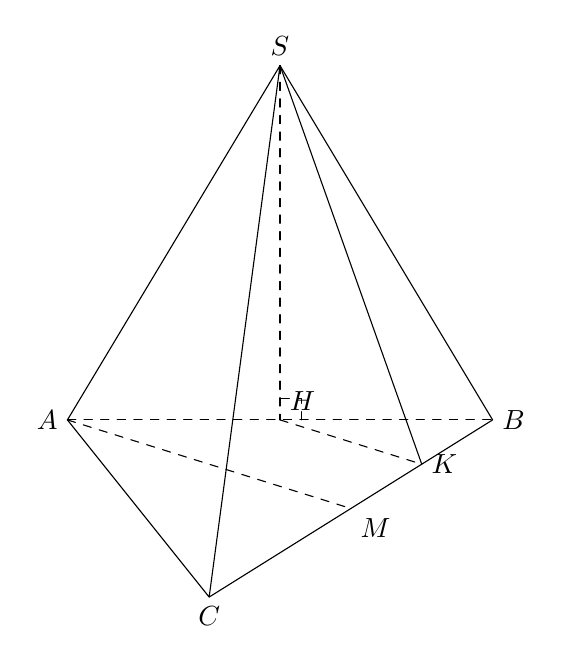
\begin{tikzpicture}[scale=0.9, line join=round, line cap=round]
				\coordinate (A) at (0,0);
				\coordinate (B) at (6,0);
				\coordinate (C) at (2,-2.5);
				\coordinate (H) at (3,0);
				\coordinate (S) at (3,5);
				\coordinate (M) at (4,-1.25);
				\coordinate (K) at (5,-0.625);
				
				\draw[dashed] (A) -- (B);
				\draw[dashed] (S) -- (H);
				\draw[dashed] (A) -- (M);
				\draw[dashed] (H) -- (K);
				\draw (S) -- (A) -- (C) -- (B) -- (S) -- (C);
				\draw (S) -- (K);
				
				\node[left] at (A) {$A$};
				\node[right] at (B) {$B$};
				\node[below] at (C) {$C$};
				\node[above] at (S) {$S$};
				\node[above right] at (H) {$H$};
				\node[right] at (K) {$K$};
				\node[below right] at (M) {$M$};
				
				% Kí hiệu vuông góc tại H
				\draw[dashed] (3.3,0) -- (3.3,0.3) -- (3,0.3);
			\end{tikzpicture}
		\end{center}
		Gọi $H$ là trung điểm của $AB$. Theo giả thiết, $SH \perp \left( ABC \right)$. \\
		Diện tích đáy là tam giác đều cạnh $a = 6$: 
		$$S_{\triangle ABC} = \dfrac{6^2\sqrt{3}}{4} = 9\sqrt{3}.$$
		Kẻ $AM \perp BC$ tại $M$, suy ra $M$ là trung điểm của $BC$ và $AM = \dfrac{6\sqrt{3}}{2} = 3\sqrt{3}$. \\
		Trong mặt phẳng $\left( ABC \right)$, kẻ $HK \perp BC$ tại $K$. \\
		Vì $\begin{cases} BC \perp HK \\ BC \perp SH \end{cases} \implies BC \perp \left( SHK \right) \implies BC \perp SK$. \\
		Ta có $\begin{cases} \left( SBC \right) \cap \left( ABC \right) = BC \\ SK \subset \left( SBC \right), SK \perp BC \\ HK \subset \left( ABC \right), HK \perp BC \end{cases}$ \\
		Suy ra góc phẳng nhị diện $\left[ S, BC, A \right]$ chính là góc $\widehat{SKH} = 60^\circ$. \\
		Trong $\triangle ABM$, ta có $H$ là trung điểm $AB$ và $HK \parallel AM$ (cùng vuông góc với $BC$) nên $HK$ là đường trung bình của $\triangle ABM$. \\
		Suy ra $K$ là trung điểm của $BM$ và $HK = \dfrac{1}{2}AM = \dfrac{3\sqrt{3}}{2}$. \\
		Xét tam giác $SHK$ vuông tại $H$:
		$$SH = HK \cdot \tan \widehat{SKH} = \dfrac{3\sqrt{3}}{2} \cdot \tan 60^\circ = \dfrac{3\sqrt{3}}{2} \cdot \sqrt{3} = \dfrac{9}{2}.$$
		Thể tích khối chóp $S.ABC$ là:
		$$V = \dfrac{1}{3} \cdot S_{\triangle ABC} \cdot SH = \dfrac{1}{3} \cdot 9\sqrt{3} \cdot \dfrac{9}{2} = \dfrac{27\sqrt{3}}{2}.$$
		Giá trị xấp xỉ: $V = \dfrac{27\sqrt{3}}{2} \approx 23,38268...$ \\
		Làm tròn kết quả đến hàng phần mười, ta được $V \approx 23,4$.
	}
\end{ex}


\begin{ex}%[1D6V4-6]
	Vào ngày $15$ tháng $1$ năm $2026$ anh Bình gửi vào ngân hàng $1$ tỷ đồng với lãi suất $0,6\%$/tháng. Kể từ tháng $2$ năm $2026$, cứ vào ngày $15$ mỗi tháng anh Bình đến ngân hàng rút ra $25$ triệu đồng để chi tiêu. Hỏi sau bao nhiêu tháng anh Bình rút hết tiền trong ngân hàng $\left( \text{ở tháng cuối cùng, số tiền rút ra có thể ít hơn } 25 \text{ triệu đồng} \right)$.
	\par\shortans{46}
	\loigiai{
		Đây là bài toán gửi tiền một lần và rút tiền định kỳ hàng tháng.
		Gọi $P$ là số tiền ban đầu gửi vào ngân hàng $\left( P = 1 \text{ tỷ đồng} = 1000 \text{ triệu đồng} \right)$.
		Gọi $r$ là lãi suất hàng tháng $\left( r = 0,6\% = 0,006 \right)$.
		Gọi $X$ là số tiền rút ra hàng tháng $\left( X = 25 \text{ triệu đồng} \right)$.
		Gọi $S_n$ là số tiền còn lại trong ngân hàng sau tháng thứ $n$ $\left( \text{ngay sau khi rút tiền lần thứ } n \right)$. Quá trình tính toán diễn ra như sau:
		\begin{itemize}
			\item Sau tháng thứ $1$, số tiền còn lại là: $S_1 = P\left( 1+r \right) - X$.
			\item Sau tháng thứ $2$, số tiền còn lại là: $S_2 = S_1\left( 1+r \right) - X = P\left( 1+r \right)^2 - X\left( 1+r \right) - X$.
			\item Tương tự, sau tháng thứ $n$, số tiền còn lại là: 
			$S_n = P\left( 1+r \right)^n - X\left[ \left( 1+r \right)^{n-1} + \left( 1+r \right)^{n-2} + ... + 1 \right]$
			Áp dụng công thức tổng của cấp số nhân cho biểu thức trong ngoặc vuông, ta có:
			$S_n = P\left( 1+r \right)^n - X\dfrac{\left( 1+r \right)^n - 1}{r}$.
		\end{itemize}
		Để anh Bình rút hết tiền trong ngân hàng thì số dư sau cùng phải nhỏ hơn hoặc bằng $0$, tức là $S_n \le 0$.
		$\Leftrightarrow P\left( 1+r \right)^n - X\dfrac{\left( 1+r \right)^n - 1}{r} \le 0$
		$\Leftrightarrow P \cdot r\left( 1+r \right)^n \le X\left( 1+r \right)^n - X$
		$\Leftrightarrow \left( 1+r \right)^n \left( X - P \cdot r \right) \ge X$
		$\Leftrightarrow \left( 1+r \right)^n \ge \dfrac{X}{X - P \cdot r}$
		
		Thay các giá trị $P = 1000, r = 0,006, X = 25$ vào bất phương trình, ta được:
		$\left( 1 + 0,006 \right)^n \ge \dfrac{25}{25 - 1000 \cdot 0,006}$
		$\Leftrightarrow 1,006^n \ge \dfrac{25}{25 - 6}$
		$\Leftrightarrow 1,006^n \ge \dfrac{25}{19}$
		$\Leftrightarrow n \ge \log_{1,006}\left( \dfrac{25}{19} \right)$
		$\Leftrightarrow n \ge 45,876...$
		
		Vì $n$ là số tháng nên $n$ phải là số nguyên dương. Do đó, ta chọn giá trị nguyên dương nhỏ nhất thỏa mãn là $n = 46$.
		Vậy sau $46$ tháng thì anh Bình sẽ rút hết tiền trong ngân hàng.
	}
\end{ex}

\begin{ex}%[0D0V2-3]
	Cho một bảng ô vuông kích thước $2 \times 7$ như hình vẽ dưới đây.
	\begin{center}
		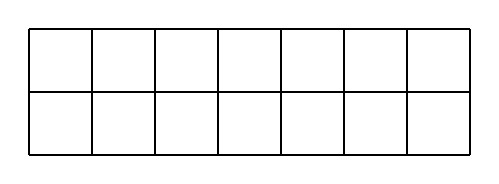
\begin{tikzpicture}[scale=0.8]
			\draw[thick] (0,0) grid (7,2);
		\end{tikzpicture}
	\end{center}
	Hai ô vuông gọi là kề nhau nếu có chung một cạnh. Người ta tô màu các ô vuông bởi hai màu đen và đỏ sao cho mỗi ô chỉ được tô đúng một màu. Gọi $P$ là xác suất để có đúng $3$ ô được tô màu đỏ và không có hai ô đỏ nào kề nhau. Giá trị $8192P$ bằng bao nhiêu?
	\par\shortans{85}
	\loigiai{
		Số phần tử của không gian mẫu (số cách tô màu ngẫu nhiên $14$ ô vuông bằng $2$ màu đen và đỏ) là:
		$$n\left( \Omega \right) = 2^{14} = 16384.$$
		Gọi $A$ là biến cố: ``Có đúng $3$ ô được tô màu đỏ và không có hai ô đỏ nào kề nhau''. \\
		Ta cần chọn $3$ ô màu đỏ thỏa mãn điều kiện. Do bảng có kích thước $2 \times 7$, hai ô trên cùng một cột luôn kề nhau nên $3$ ô màu đỏ phải nằm ở $3$ cột khác nhau trong $7$ cột của bảng. \\
		Chia các trường hợp chọn $3$ cột chứa ô màu đỏ:
		\begin{itemize}
			\item \textbf{Trường hợp 1:} $3$ cột chứa ô đỏ rời nhau hoàn toàn (không có bất kỳ hai cột nào kề nhau). \\
			Số cách chọn $3$ cột từ $7$ cột sao cho không có $2$ cột kề nhau là $\mathrm{C}_{7-3+1}^{3} = \mathrm{C}_{5}^{3} = 10$ cách. \\
			Với mỗi cột được chọn, có $2$ cách chọn ô màu đỏ (dòng trên hoặc dòng dưới). \\
			Số cách tô màu trong trường hợp này là: $10 \cdot 2^3 = 80$ cách.
			
			\item \textbf{Trường hợp 2:} $3$ cột chứa ô đỏ có đúng $2$ cột kề nhau. \\
			Số cách chọn $3$ cột bất kỳ là $\mathrm{C}_{7}^{3} = 35$ cách. \\
			Số cách chọn $3$ cột liền kề nhau là $5$ cách (gồm các bộ $\{1,2,3\}, \{2,3,4\}, \{3,4,5\}, \{4,5,6\}, \{5,6,7\}$). \\
			Suy ra số cách chọn $3$ cột có đúng $2$ cột kề nhau là $35 - 10 - 5 = 20$ cách. \\
			Đối với $2$ cột kề nhau, để $2$ ô đỏ không kề nhau thì phải chọn khác dòng ($2$ cách: trên-dưới hoặc dưới-trên). Cột rời còn lại có $2$ cách chọn ô đỏ. \\
			Số cách tô màu trong trường hợp này là: $20 \cdot 2 \cdot 2 = 80$ cách.
			
			\item \textbf{Trường hợp 3:} $3$ cột chứa ô đỏ liền kề nhau. \\
			Có $5$ cách chọn bộ $3$ cột liền kề. \\
			Để các ô đỏ không kề nhau, ta phải chọn các ô đỏ xen kẽ dòng (trên-dưới-trên hoặc dưới-trên-dưới), tức là có $2$ cách chọn cho mỗi bộ. \\
			Số cách tô màu trong trường hợp này là: $5 \cdot 2 = 10$ cách.
		\end{itemize}
		Số kết quả thuận lợi cho biến cố $A$ là:
		$$n\left( A \right) = 80 + 80 + 10 = 170.$$
		Xác suất của biến cố $A$ là:
		$$P = \dfrac{n\left( A \right)}{n\left( \Omega \right)} = \dfrac{170}{16384} = \dfrac{85}{8192}.$$
		Vậy giá trị của $8192P$ là:
		$$8192P = 8192 \cdot \dfrac{85}{8192} = 85.$$
	}
\end{ex}

\begin{ex}%[2D1H3-6]
	Một doanh nghiệp dự định sản xuất không quá $200$ đơn vị sản phẩm. Nếu doanh nghiệp sản xuất $x$ đơn vị sản phẩm $\left( 1 \le x \le 200 \right)$ thì giá bán của mỗi đơn vị sản phẩm là $f\left( x \right) = 435 - 2x$ (triệu đồng) và chi phí sản xuất bình quân cho một đơn vị sản phẩm là $g\left( x \right) = \dfrac{0,7x^2}{125} - 1,706x + 96,5 + \dfrac{6375}{x}$ (triệu đồng). Biết rằng mức thuế cho một đơn vị sản phẩm này là $2,5$ triệu đồng. Hỏi doanh nghiệp cần sản xuất bao nhiêu đơn vị sản phẩm để lợi nhuận thu được lớn nhất?
	\par\shortans{125}
	\loigiai{
		Gọi $x$ là số đơn vị sản phẩm doanh nghiệp sản xuất $\left( 1 \le x \le 200, x \in \mathbb{N} \right)$. \\
		Tổng doanh thu khi bán $x$ sản phẩm là:
		$$R\left( x \right) = x \cdot f\left( x \right) = x \left( 435 - 2x \right) = -2x^2 + 435x.$$
		Tổng chi phí sản xuất $x$ sản phẩm (bao gồm cả thuế) là:
		$$C\left( x \right) = x \cdot g\left( x \right) + 2,5x = x \left( \dfrac{0,7x^2}{125} - 1,706x + 96,5 + \dfrac{6375}{x} \right) + 2,5x$$
		$$C\left( x \right) = \dfrac{0,7x^3}{125} - 1,706x^2 + 96,5x + 6375 + 2,5x = 0,0056x^3 - 1,706x^2 + 99x + 6375.$$
		Hàm lợi nhuận của doanh nghiệp là $P\left( x \right) = R\left( x \right) - C\left( x \right)$:
		$$P\left( x \right) = -2x^2 + 435x - \left( 0,0056x^3 - 1,706x^2 + 99x + 6375 \right)$$
		$$P\left( x \right) = -0,0056x^3 - 0,294x^2 + 336x - 6375.$$
		Ta tìm giá trị lớn nhất của hàm số $P\left( x \right)$ trên đoạn $\left[ 1; 200 \right]$. \\
		Đạo hàm $P'\left( x \right) = -0,0168x^2 - 0,588x + 336$. \\
		Cho $P'\left( x \right) = 0 \Leftrightarrow -0,0168x^2 - 0,588x + 336 = 0 \Leftrightarrow x^2 + 35x - 20000 = 0$. \\
		Giải phương trình bậc hai ta được:
		$$ \left[ \begin{array}{l} x = 125 \text{ (thỏa mãn } x \in \left[ 1; 200 \right] \text{)} \\ x = -160 \text{ (loại)} \end{array} \right. $$
		Vì $P''\left( x \right) = -0,0336x - 0,588 \implies P''\left( 125 \right) < 0$ nên hàm số đạt cực đại tại $x = 125$. \\
		Trên đoạn $\left[ 1; 200 \right]$, hàm số chỉ có một điểm cực đại duy nhất là $x = 125$ nên lợi nhuận đạt giá trị lớn nhất tại đây. \\
		Vậy doanh nghiệp cần sản xuất $125$ đơn vị sản phẩm để thu được lợi nhuận lớn nhất.
	}
\end{ex}

\begin{ex}%[2D4V3-5]
	\immini{
	Một mô hình khối tròn xoay có trục là đường thẳng $MN$, khi ta cắt khối tròn xoay đó bởi một mặt phẳng đi qua trục của khối tròn xoay thì ta được mặt cắt có dạng như hình vẽ dưới đây.\\
	\noindent Biết $MN = 24$ cm, $ABCD$ là hình chữ nhật có $AB = 18$ cm, $AD = 36$ cm, hai cung $APD$ và $BQC$ là một phần của các đường parabol với đỉnh lần lượt là $P, Q$ và $PQ = 10$ cm. Thể tích của mô hình đó bằng bao nhiêu xăng-ti-mét khối (kết quả làm tròn đến hàng đơn vị)?
	}{
		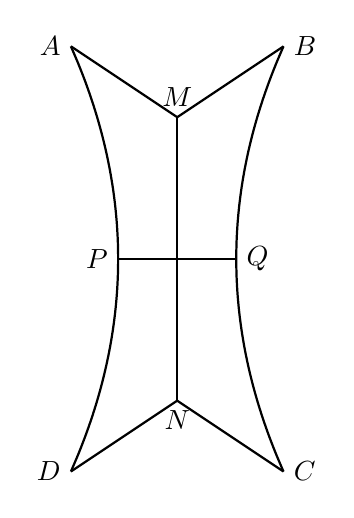
\begin{tikzpicture}[scale=0.15, thick]
			\coordinate (A) at (-9, 18);
			\coordinate (B) at (9, 18);
			\coordinate (C) at (9, -18);
			\coordinate (D) at (-9, -18);
			\coordinate (M) at (0, 12);
			\coordinate (N) at (0, -12);
			\coordinate (P) at (-5, 0);
			\coordinate (Q) at (5, 0);
			
			% Parabol branches
			\draw[domain=-18:18, smooth, variable=\y] plot ({-(\y*\y)/81 - 5}, {\y});
			\draw[domain=-18:18, smooth, variable=\y] plot ({\y*\y/81 + 5}, {\y});
			
			% Straight segments
			\draw (A) -- (M) -- (B);
			\draw (D) -- (N) -- (C);
			\draw (M) -- (N);
			\draw (P) -- (Q);
			
			% Labels
			\node[left] at (A) {$A$};
			\node[right] at (B) {$B$};
			\node[right] at (C) {$C$};
			\node[left] at (D) {$D$};
			\node[above] at (M) {$M$};
			\node[below] at (N) {$N$};
			\node[left] at (P) {$P$};
			\node[right] at (Q) {$Q$};
		\end{tikzpicture}
	}
	\par\shortans{3679}
	\loigiai{
		Chọn hệ trục tọa độ $Oxy$ sao cho gốc $O$ là tâm của hình chữ nhật $ABCD$, trục $Oy$ chứa đoạn thẳng $MN$ và trục $Ox$ chứa đoạn thẳng $PQ$.
		
		Khi đó, mặt cắt nằm trong mặt phẳng $Oxy$ với tọa độ các điểm như sau:
		\begin{itemize}
			\item Chiều cao $AD = 36 \implies$ Tung độ của $B, A$ là $18$ và của $C, D$ là $-18$.
			\item Chiều rộng $AB = 18 \implies$ Hoành độ của $B, C$ là $9$. Do đó $B\left( 9; 18 \right)$ và $C\left( 9; -18 \right)$.
			\item $PQ = 10 \implies$ Đỉnh parabol bên phải là $Q\left( 5; 0 \right)$.
			\item $MN = 24 \implies M\left( 0; 12 \right)$ và $N\left( 0; -12 \right)$.
		\end{itemize}
		
		Phương trình parabol chứa cung $BQC$ có đỉnh $Q\left( 5; 0 \right)$ nằm trên trục hoành có dạng $x = ay^2 + 5$. \\
		Vì parabol đi qua điểm $B\left( 9; 18 \right)$ nên ta có:
		$$9 = a \cdot 18^2 + 5 \Leftrightarrow a = \dfrac{4}{324} = \dfrac{1}{81}.$$
		Suy ra phương trình parabol là $x = \dfrac{y^2}{81} + 5$.
		
		Phần thể tích của mô hình khối tròn xoay này bằng thể tích khối tròn xoay được tạo thành khi quay miền phẳng ở bên phải trục tung giới hạn bởi trục $Oy$, parabol $x = \dfrac{y^2}{81} + 5$, và các đoạn thẳng $MB$, $NC$ quanh trục $Oy$.
		
		Ta có thể tính thể tích $V$ của mô hình bằng cách lấy thể tích khối tròn xoay sinh bởi hình phẳng giới hạn bởi đường parabol $x = \dfrac{y^2}{81} + 5$, $y = 18, y = -18$ và trục $Oy$ (gọi là $V_1$), trừ đi thể tích sinh bởi hai phần khuyết ở trên và dưới (là hai khối nón bằng nhau sinh bởi tam giác vuông giới hạn bởi $MB$ và $NC$ khi quay quanh $Oy$, gọi tổng thể tích này là $V_2$).
		
		Thể tích $V_1$ được tính bằng công thức:
		$$V_1 = \pi \int_{-18}^{18} \left( \dfrac{y^2}{81} + 5 \right)^2 \mathrm{d}y = 2\pi \int_{0}^{18} \left( \dfrac{y^4}{6561} + \dfrac{10y^2}{81} + 25 \right) \mathrm{d}y$$
		$$V_1 = 2\pi \left[ \dfrac{y^5}{32805} + \dfrac{10y^3}{243} + 25y \right]_{0}^{18} = 2\pi \left( \dfrac{288}{5} + 240 + 450 \right) = \dfrac{7476\pi}{5} = 1495,2\pi.$$
		
		Hai phần khuyết khi quay tạo thành hai khối nón có cùng bán kính đáy $R = 9$ (do hoành độ của điểm $B$ và $C$ đều bằng $9$) và chiều cao $h = 18 - 12 = 6$.
		Thể tích hai khối nón này là:
		$$V_2 = 2 \cdot \left( \dfrac{1}{3} \pi R^2 h \right) = 2 \cdot \dfrac{1}{3} \pi \cdot 9^2 \cdot 6 = 324\pi.$$
		
		Thể tích của toàn bộ mô hình khối tròn xoay là:
		$$V = V_1 - V_2 = 1495,2\pi - 324\pi = 1171,2\pi.$$
		
		Giá trị xấp xỉ của thể tích là:
		$$V \approx 1171,2 \cdot 3,14159265 \approx 3679,43.$$
		Làm tròn kết quả đến hàng đơn vị, ta được $3679$ cm$^3$.
	}
\end{ex}

\begin{ex}%[0D8V2-2]
	\immini{
	Cho tập hợp gồm $18$ số tự nhiên $S=\left\{ 1; 2; 3; 4; 5; 6; 7; 8; 9; 10; 11; 12; 13; 14; 15; 16; 17; 18 \right\}$. Chọn ngẫu nhiên $9$ số tự nhiên từ tập và điền vào $9$ ô vuông của một bảng $3\times 3$ như hình vẽ. Gọi $T$ là số cách điền thỏa mãn hai đường chéo theo thứ tự lập thành cấp số nhân. Tính giá trị $\dfrac{T}{100}$.
	}{
		
\begin{tikzpicture}[line width=1.5pt, scale=1.2]
			\draw (0,0) grid (3,3);
		\end{tikzpicture}
	}
	\par\shortans{6864}
	\loigiai{
		Giả sử $9$ ô vuông của bảng được điền các số $a_{ij}$ với $i,j \in \left\{ 1; 2; 3 \right\}$.
		Hai đường chéo của bảng là $\left( a_{11}, a_{22}, a_{33} \right)$ và $\left( a_{13}, a_{22}, a_{31} \right)$, chúng có chung phần tử ở chính giữa là $a_{22}$.
		Vì mỗi đường chéo theo thứ tự lập thành một cấp số nhân nên ta có:
		$a_{22}^2 = a_{11} \cdot a_{33} = a_{13} \cdot a_{31}$.
		Do $9$ số được điền phân biệt và lấy từ tập $S$, nên $a_{22}$ phải là số mà bình phương của nó có thể phân tích được thành ít nhất $2$ tích của các cặp số phân biệt trong $S$ $\left( \text{các số này cũng phải khác } a_{22} \right)$.
		Ta xét các trường hợp có thể của phần tử trung tâm $a_{22} \in S$:
		\begin{itemize}
			\item Nếu $a_{22} = 4 \Rightarrow a_{22}^2 = 16$. Ta có các cặp phân tích hợp lệ: $\left\{ 1; 16 \right\}$ và $\left\{ 2; 8 \right\}$.
			Số cách chọn $2$ cặp số là $\mathrm{C}_{2}^{2} = 1$ cách.
			Số cách phân bổ $2$ cặp số vào $2$ đường chéo là $2$ cách.
			Mỗi cặp số trên một đường chéo có $2$ cách hoán vị. Suy ra có $1 \cdot 2 \cdot 2 \cdot 2 = 8$ cách điền số cho $5$ ô trên $2$ đường chéo.
			
			\item Nếu $a_{22} = 6 \Rightarrow a_{22}^2 = 36$. Ta có các cặp phân tích hợp lệ: $\left\{ 2; 18 \right\}$, $\left\{ 3; 12 \right\}$ và $\left\{ 4; 9 \right\}$.
			Số cách chọn $2$ cặp số trong $3$ cặp là $\mathrm{C}_{3}^{2} = 3$ cách.
			Tương tự trường hợp trên, số cách điền số cho $5$ ô trên $2$ đường chéo là $3 \cdot 2 \cdot 2 \cdot 2 = 24$ cách.
			
			\item Nếu $a_{22} = 12 \Rightarrow a_{22}^2 = 144$. Ta có các cặp phân tích hợp lệ: $\left\{ 8; 18 \right\}$ và $\left\{ 9; 16 \right\}$.
			Số cách chọn $2$ cặp số là $\mathrm{C}_{2}^{2} = 1$ cách.
			Tương tự, số cách điền số cho $5$ ô trên $2$ đường chéo là $1 \cdot 2 \cdot 2 \cdot 2 = 8$ cách.
		\end{itemize}
		Các giá trị khác của $a_{22}$ không có đủ ít nhất $2$ cặp số hợp lệ thỏa mãn điều kiện bài toán.
		Tổng số cách điền số vào $5$ ô trên $2$ đường chéo là $8 + 24 + 8 = 40$ cách.
		Sau khi đã điền $5$ ô trên, ta còn $18 - 5 = 13$ số chưa sử dụng.
		Số cách chọn $4$ số từ $13$ số này và sắp xếp vào $4$ ô còn trống của bảng là: 
		$13 \cdot 12 \cdot 11 \cdot 10 = 17160$ $\left( \text{cách} \right)$.
		Vậy tổng số cách điền bảng thỏa mãn yêu cầu bài toán là $T = 40 \cdot 17160 = 686400$.
		Giá trị cần tính là $\dfrac{T}{100} = \dfrac{686400}{100} = 6864$.
	}
\end{ex}


\Closesolutionfile{ans}

%\indapan{6}{ans/ans-04-26-2-QuangNinh-SoGD-LC}
%\indapan{4}{ans/ans-04-26-2-QuangNinh-SoGD-DS}
%\indapan{6}{ans/ans-04-26-2-QuangNinh-SoGD-KQ}